\documentclass[1p]{elsarticle_modified}
%\bibliographystyle{elsarticle-num}

%\usepackage[colorlinks]{hyperref}
%\usepackage{abbrmath_seonhwa} %\Abb, \Ascr, \Acal ,\Abf, \Afrak
\usepackage{amsfonts}
\usepackage{amssymb}
\usepackage{amsmath}
\usepackage{amsthm}
\usepackage{scalefnt}
\usepackage{amsbsy}
\usepackage{kotex}
\usepackage{caption}
\usepackage{subfig}
\usepackage{color}
\usepackage{graphicx}
\usepackage{xcolor} %% white, black, red, green, blue, cyan, magenta, yellow
\usepackage{float}
\usepackage{setspace}
\usepackage{hyperref}

\usepackage{tikz}
\usetikzlibrary{arrows}

\usepackage{multirow}
\usepackage{array} % fixed length table
\usepackage{hhline}

%%%%%%%%%%%%%%%%%%%%%
\makeatletter
\renewcommand*\env@matrix[1][\arraystretch]{%
	\edef\arraystretch{#1}%
	\hskip -\arraycolsep
	\let\@ifnextchar\new@ifnextchar
	\array{*\c@MaxMatrixCols c}}
\makeatother %https://tex.stackexchange.com/questions/14071/how-can-i-increase-the-line-spacing-in-a-matrix
%%%%%%%%%%%%%%%

\usepackage[normalem]{ulem}

\newcommand{\msout}[1]{\ifmmode\text{\sout{\ensuremath{#1}}}\else\sout{#1}\fi}
%SOURCE: \msout is \stkout macro in https://tex.stackexchange.com/questions/20609/strikeout-in-math-mode

\newcommand{\cancel}[1]{
	\ifmmode
	{\color{red}\msout{#1}}
	\else
	{\color{red}\sout{#1}}
	\fi
}

\newcommand{\add}[1]{
	{\color{blue}\uwave{#1}}
}

\newcommand{\replace}[2]{
	\ifmmode
	{\color{red}\msout{#1}}{\color{blue}\uwave{#2}}
	\else
	{\color{red}\sout{#1}}{\color{blue}\uwave{#2}}
	\fi
}

\newcommand{\Sol}{\mathcal{S}} %segment
\newcommand{\D}{D} %diagram
\newcommand{\A}{\mathcal{A}} %arc


%%%%%%%%%%%%%%%%%%%%%%%%%%%%%5 test

\def\sl{\operatorname{\textup{SL}}(2,\Cbb)}
\def\psl{\operatorname{\textup{PSL}}(2,\Cbb)}
\def\quan{\mkern 1mu \triangleright \mkern 1mu}

\theoremstyle{definition}
\newtheorem{thm}{Theorem}[section]
\newtheorem{prop}[thm]{Proposition}
\newtheorem{lem}[thm]{Lemma}
\newtheorem{ques}[thm]{Question}
\newtheorem{cor}[thm]{Corollary}
\newtheorem{defn}[thm]{Definition}
\newtheorem{exam}[thm]{Example}
\newtheorem{rmk}[thm]{Remark}
\newtheorem{alg}[thm]{Algorithm}

\newcommand{\I}{\sqrt{-1}}
\begin{document}

%\begin{frontmatter}
%
%\title{Boundary parabolic representations of knots up to 8 crossings}
%
%%% Group authors per affiliation:
%\author{Yunhi Cho} 
%\address{Department of Mathematics, University of Seoul, Seoul, Korea}
%\ead{yhcho@uos.ac.kr}
%
%
%\author{Seonhwa Kim} %\fnref{s_kim}}
%\address{Center for Geometry and Physics, Institute for Basic Science, Pohang, 37673, Korea}
%\ead{ryeona17@ibs.re.kr}
%
%\author{Hyuk Kim}
%\address{Department of Mathematical Sciences, Seoul National University, Seoul 08826, Korea}
%\ead{hyukkim@snu.ac.kr}
%
%\author{Seokbeom Yoon}
%\address{Department of Mathematical Sciences, Seoul National University, Seoul, 08826,  Korea}
%\ead{sbyoon15@snu.ac.kr}
%
%\begin{abstract}
%We find all boundary parabolic representation of knots up to 8 crossings.
%
%\end{abstract}
%\begin{keyword}
%    \MSC[2010] 57M25 
%\end{keyword}
%
%\end{frontmatter}

%\linenumbers
%\tableofcontents
%
\newcommand\colored[1]{\textcolor{white}{\rule[-0.35ex]{0.8em}{1.4ex}}\kern-0.8em\color{red} #1}%
%\newcommand\colored[1]{\textcolor{white}{ #1}\kern-2.17ex	\textcolor{white}{ #1}\kern-1.81ex	\textcolor{white}{ #1}\kern-2.15ex\color{red}#1	}

{\Large $\underline{12a_{0835}~(K12a_{0835})}$}

\setlength{\tabcolsep}{10pt}
\renewcommand{\arraystretch}{1.6}
\vspace{1cm}\begin{tabular}{m{100pt}>{\centering\arraybackslash}m{274pt}}
\multirow{5}{120pt}{
	\centering
	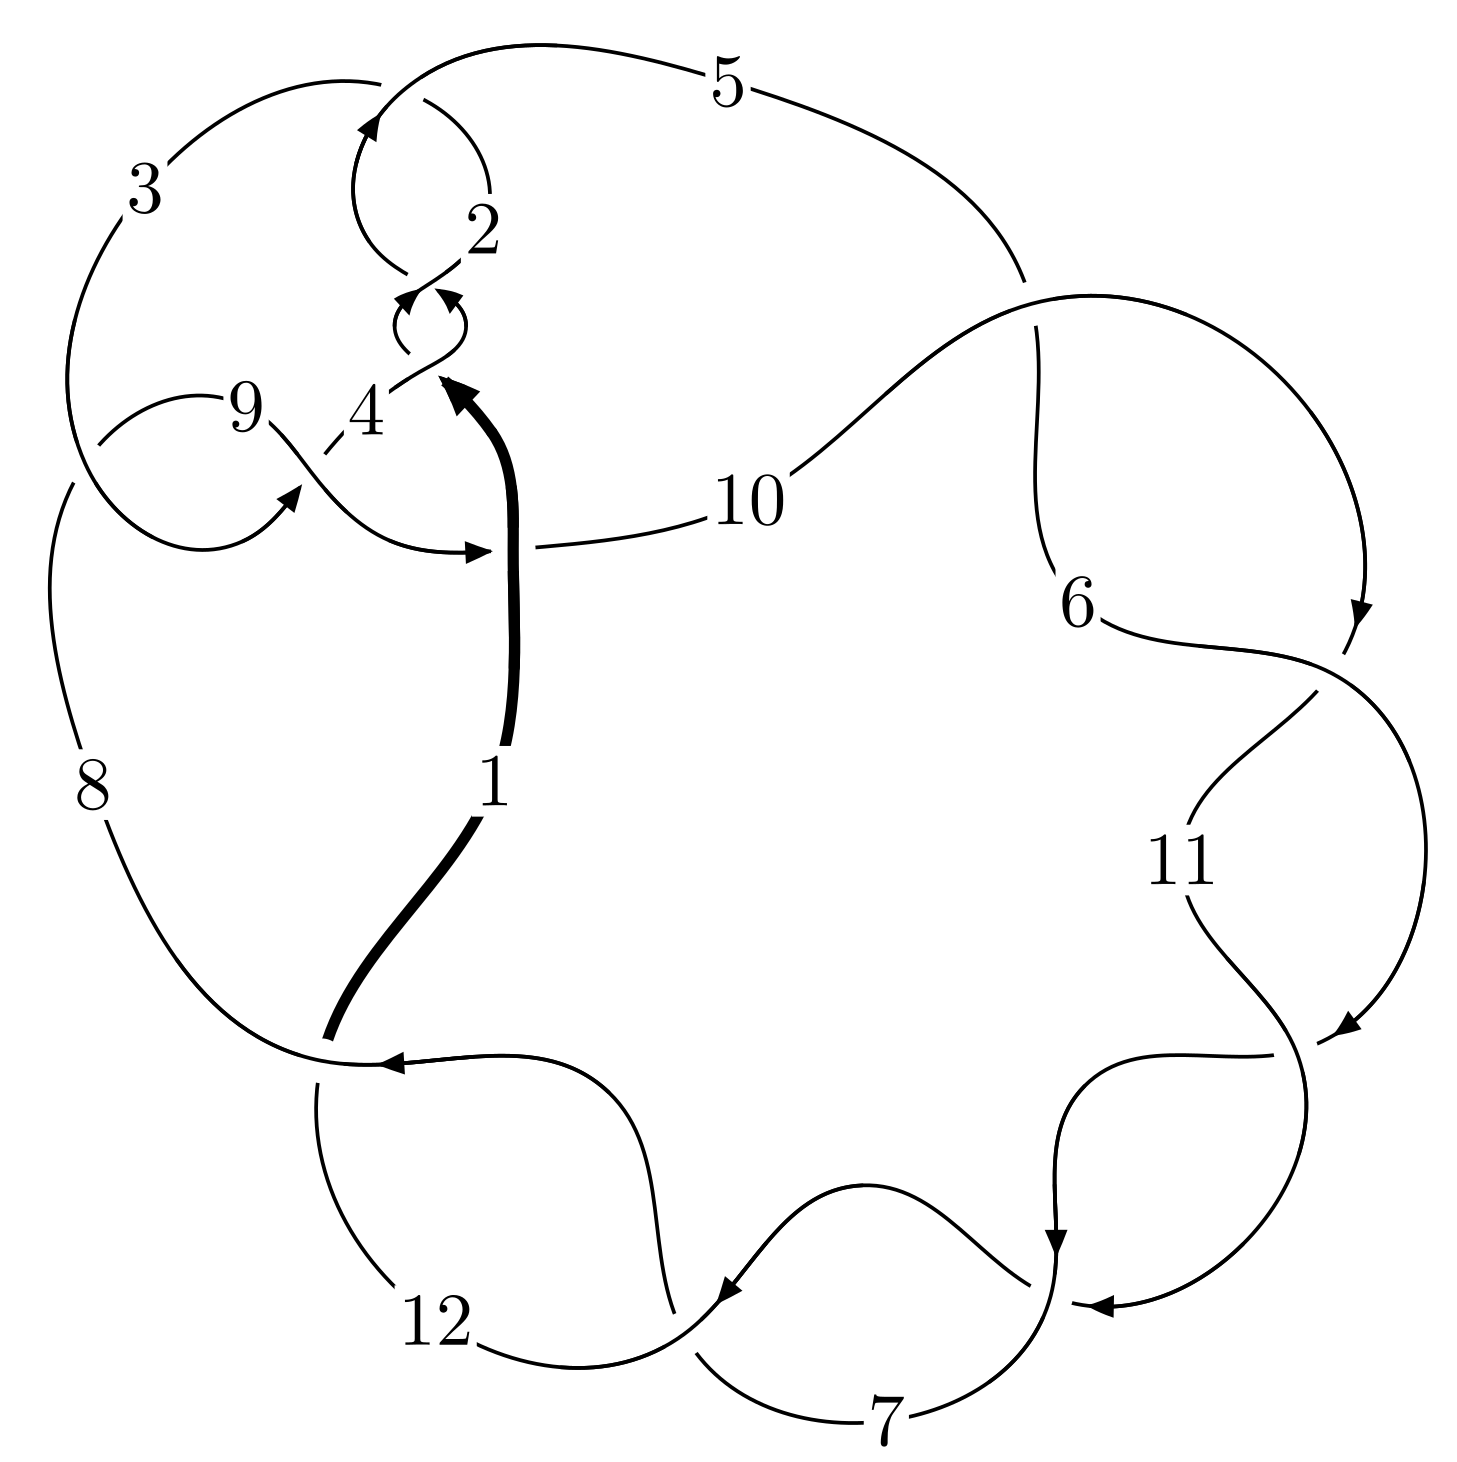
\includegraphics[width=112pt]{../../../GIT/diagram.site/Diagrams/png/1636_12a_0835.png}\\
\ \ \ A knot diagram\footnotemark}&
\allowdisplaybreaks
\textbf{Linearized knot diagam} \\
\cline{2-2}
 &
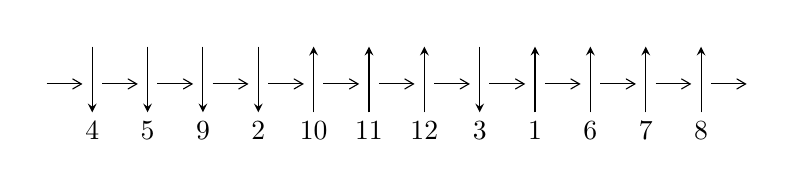
\begin{tikzpicture}[x=20pt, y=17pt]
	% nodes
	\node (C0) at (0, 0) {};
	\node (C1) at (1, 0) {};
	\node (C1U) at (1, +1) {};
	\node (C1D) at (1, -1) {4};

	\node (C2) at (2, 0) {};
	\node (C2U) at (2, +1) {};
	\node (C2D) at (2, -1) {5};

	\node (C3) at (3, 0) {};
	\node (C3U) at (3, +1) {};
	\node (C3D) at (3, -1) {9};

	\node (C4) at (4, 0) {};
	\node (C4U) at (4, +1) {};
	\node (C4D) at (4, -1) {2};

	\node (C5) at (5, 0) {};
	\node (C5U) at (5, +1) {};
	\node (C5D) at (5, -1) {10};

	\node (C6) at (6, 0) {};
	\node (C6U) at (6, +1) {};
	\node (C6D) at (6, -1) {11};

	\node (C7) at (7, 0) {};
	\node (C7U) at (7, +1) {};
	\node (C7D) at (7, -1) {12};

	\node (C8) at (8, 0) {};
	\node (C8U) at (8, +1) {};
	\node (C8D) at (8, -1) {3};

	\node (C9) at (9, 0) {};
	\node (C9U) at (9, +1) {};
	\node (C9D) at (9, -1) {1};

	\node (C10) at (10, 0) {};
	\node (C10U) at (10, +1) {};
	\node (C10D) at (10, -1) {6};

	\node (C11) at (11, 0) {};
	\node (C11U) at (11, +1) {};
	\node (C11D) at (11, -1) {7};

	\node (C12) at (12, 0) {};
	\node (C12U) at (12, +1) {};
	\node (C12D) at (12, -1) {8};
	\node (C13) at (13, 0) {};

	% arrows
	\draw[->,>={angle 60}]
	(C0) edge (C1) (C1) edge (C2) (C2) edge (C3) (C3) edge (C4) (C4) edge (C5) (C5) edge (C6) (C6) edge (C7) (C7) edge (C8) (C8) edge (C9) (C9) edge (C10) (C10) edge (C11) (C11) edge (C12) (C12) edge (C13) ;	\draw[->,>=stealth]
	(C1U) edge (C1D) (C2U) edge (C2D) (C3U) edge (C3D) (C4U) edge (C4D) (C5D) edge (C5U) (C6D) edge (C6U) (C7D) edge (C7U) (C8U) edge (C8D) (C9D) edge (C9U) (C10D) edge (C10U) (C11D) edge (C11U) (C12D) edge (C12U) ;
	\end{tikzpicture} \\
\hhline{~~} \\& 
\textbf{Solving Sequence} \\ \cline{2-2} 
 &
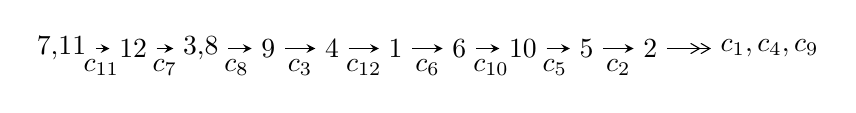
\begin{tikzpicture}[x=23pt, y=7pt]
	% node
	\node (A0) at (-1/8, 0) {7,11};
	\node (A1) at (1, 0) {12};
	\node (A2) at (33/16, 0) {3,8};
	\node (A3) at (25/8, 0) {9};
	\node (A4) at (33/8, 0) {4};
	\node (A5) at (41/8, 0) {1};
	\node (A6) at (49/8, 0) {6};
	\node (A7) at (57/8, 0) {10};
	\node (A8) at (65/8, 0) {5};
	\node (A9) at (73/8, 0) {2};
	\node (C1) at (1/2, -1) {$c_{11}$};
	\node (C2) at (3/2, -1) {$c_{7}$};
	\node (C3) at (21/8, -1) {$c_{8}$};
	\node (C4) at (29/8, -1) {$c_{3}$};
	\node (C5) at (37/8, -1) {$c_{12}$};
	\node (C6) at (45/8, -1) {$c_{6}$};
	\node (C7) at (53/8, -1) {$c_{10}$};
	\node (C8) at (61/8, -1) {$c_{5}$};
	\node (C9) at (69/8, -1) {$c_{2}$};
	\node (A10) at (11, 0) {$c_{1},c_{4},c_{9}$};

	% edge
	\draw[->,>=stealth]	
	(A0) edge (A1) (A1) edge (A2) (A2) edge (A3) (A3) edge (A4) (A4) edge (A5) (A5) edge (A6) (A6) edge (A7) (A7) edge (A8) (A8) edge (A9) ;
	\draw[->>,>={angle 60}]	
	(A9) edge (A10);
\end{tikzpicture} \\ 

\end{tabular} \\

\footnotetext{
The image of knot diagram is generated by the software ``\textbf{Draw programme}" developed by Andrew Bartholomew(\url{http://www.layer8.co.uk/maths/draw/index.htm\#Running-draw}), where we modified some parts for our purpose(\url{https://github.com/CATsTAILs/LinksPainter}).
}\phantom \\ \newline 
\centering \textbf{Ideals for irreducible components\footnotemark of $X_{\text{par}}$} 
 
\begin{align*}
I^u_{1}&=\langle 
-3 u^{37}+76 u^{35}+\cdots+b+1,\;2 u^{37}+u^{36}+\cdots+a-3,\;u^{38}+2 u^{37}+\cdots-4 u-1\rangle \\
I^u_{2}&=\langle 
u^2+b-1,\;a-1,\;u^3- u^2-2 u+1\rangle \\
\\
\end{align*}
\raggedright * 2 irreducible components of $\dim_{\mathbb{C}}=0$, with total 41 representations.\\
\footnotetext{All coefficients of polynomials are rational numbers. But the coefficients are sometimes approximated in decimal forms when there is not enough margin.}
\newpage
\renewcommand{\arraystretch}{1}
\centering \section*{I. $I^u_{1}= \langle -3 u^{37}+76 u^{35}+\cdots+b+1,\;2 u^{37}+u^{36}+\cdots+a-3,\;u^{38}+2 u^{37}+\cdots-4 u-1 \rangle$}
\flushleft \textbf{(i) Arc colorings}\\
\begin{tabular}{m{7pt} m{180pt} m{7pt} m{180pt} }
\flushright $a_{7}=$&$\begin{pmatrix}0\\u\end{pmatrix}$ \\
\flushright $a_{11}=$&$\begin{pmatrix}1\\0\end{pmatrix}$ \\
\flushright $a_{12}=$&$\begin{pmatrix}1\\- u^2\end{pmatrix}$ \\
\flushright $a_{3}=$&$\begin{pmatrix}-2 u^{37}- u^{36}+\cdots-15 u^2+3\\3 u^{37}-76 u^{35}+\cdots-6 u-1\end{pmatrix}$ \\
\flushright $a_{8}=$&$\begin{pmatrix}u\\- u^3+u\end{pmatrix}$ \\
\flushright $a_{9}=$&$\begin{pmatrix}u^8-5 u^6+7 u^4-4 u^2+1\\- u^{10}+6 u^8-11 u^6+6 u^4+u^2\end{pmatrix}$ \\
\flushright $a_{4}=$&$\begin{pmatrix}- u^{36}+25 u^{34}+\cdots- u+2\\- u^{37}+26 u^{35}+\cdots+u+1\end{pmatrix}$ \\
\flushright $a_{1}=$&$\begin{pmatrix}- u^2+1\\u^4-2 u^2\end{pmatrix}$ \\
\flushright $a_{6}=$&$\begin{pmatrix}- u\\u\end{pmatrix}$ \\
\flushright $a_{10}=$&$\begin{pmatrix}- u^2+1\\u^2\end{pmatrix}$ \\
\flushright $a_{5}=$&$\begin{pmatrix}u^3-2 u\\- u^3+u\end{pmatrix}$ \\
\flushright $a_{2}=$&$\begin{pmatrix}- u^{37}- u^{36}+\cdots- u+3\\u^{37}-25 u^{35}+\cdots+u^2-2 u\end{pmatrix}$\\&\end{tabular}
\flushleft \textbf{(ii) Obstruction class $= -1$}\\~\\
\flushleft \textbf{(iii) Cusp Shapes $= u^{37}+4 u^{36}+\cdots+31 u-7$}\\~\\
\newpage\renewcommand{\arraystretch}{1}
\flushleft \textbf{(iv) u-Polynomials at the component}\newline \\
\begin{tabular}{m{50pt}|m{274pt}}
Crossings & \hspace{64pt}u-Polynomials at each crossing \\
\hline $$\begin{aligned}c_{1},c_{2},c_{4}\end{aligned}$$&$\begin{aligned}
&u^{38}-4 u^{37}+\cdots- u-1
\end{aligned}$\\
\hline $$\begin{aligned}c_{3},c_{8}\end{aligned}$$&$\begin{aligned}
&u^{38}+u^{37}+\cdots+12 u+8
\end{aligned}$\\
\hline $$\begin{aligned}c_{5},c_{6},c_{7}\\c_{10},c_{11},c_{12}\end{aligned}$$&$\begin{aligned}
&u^{38}+2 u^{37}+\cdots-4 u-1
\end{aligned}$\\
\hline $$\begin{aligned}c_{9}\end{aligned}$$&$\begin{aligned}
&u^{38}-6 u^{37}+\cdots-476 u+55
\end{aligned}$\\
\hline
\end{tabular}\\~\\
\newpage\renewcommand{\arraystretch}{1}
\flushleft \textbf{(v) Riley Polynomials at the component}\newline \\
\begin{tabular}{m{50pt}|m{274pt}}
Crossings & \hspace{64pt}Riley Polynomials at each crossing \\
\hline $$\begin{aligned}c_{1},c_{2},c_{4}\end{aligned}$$&$\begin{aligned}
&y^{38}-36 y^{37}+\cdots+35 y+1
\end{aligned}$\\
\hline $$\begin{aligned}c_{3},c_{8}\end{aligned}$$&$\begin{aligned}
&y^{38}-21 y^{37}+\cdots-848 y+64
\end{aligned}$\\
\hline $$\begin{aligned}c_{5},c_{6},c_{7}\\c_{10},c_{11},c_{12}\end{aligned}$$&$\begin{aligned}
&y^{38}-54 y^{37}+\cdots-28 y+1
\end{aligned}$\\
\hline $$\begin{aligned}c_{9}\end{aligned}$$&$\begin{aligned}
&y^{38}+6 y^{37}+\cdots-132856 y+3025
\end{aligned}$\\
\hline
\end{tabular}\\~\\
\newpage\flushleft \textbf{(vi) Complex Volumes and Cusp Shapes}
$$\begin{array}{c|c|c}  
\text{Solutions to }I^u_{1}& \I (\text{vol} + \sqrt{-1}CS) & \text{Cusp shape}\\
 \hline 
\begin{aligned}
u &= \phantom{-}0.879915 + 0.280083 I \\
a &= -0.422412 + 0.001593 I \\
b &= \phantom{-}1.259570 + 0.041859 I\end{aligned}
 & -4.46594 - 0.62155 I & \phantom{-}1.23906 - 1.00554 I \\ \hline\begin{aligned}
u &= \phantom{-}0.879915 - 0.280083 I \\
a &= -0.422412 - 0.001593 I \\
b &= \phantom{-}1.259570 - 0.041859 I\end{aligned}
 & -4.46594 + 0.62155 I & \phantom{-}1.23906 + 1.00554 I \\ \hline\begin{aligned}
u &= \phantom{-}1.107830 + 0.111217 I \\
a &= \phantom{-}1.127560 + 0.838416 I \\
b &= -0.893007 - 0.188118 I\end{aligned}
 & \phantom{-}2.67127 + 0.72425 I & \phantom{-}3.65418 - 0.86134 I \\ \hline\begin{aligned}
u &= \phantom{-}1.107830 - 0.111217 I \\
a &= \phantom{-}1.127560 - 0.838416 I \\
b &= -0.893007 + 0.188118 I\end{aligned}
 & \phantom{-}2.67127 - 0.72425 I & \phantom{-}3.65418 + 0.86134 I \\ \hline\begin{aligned}
u &= -1.132560 + 0.171155 I \\
a &= \phantom{-}0.264697 - 1.114460 I \\
b &= \phantom{-}0.795265 - 0.506019 I\end{aligned}
 & \phantom{-}1.45072 - 3.23668 I & \phantom{-}4.64812 + 3.17787 I \\ \hline\begin{aligned}
u &= -1.132560 - 0.171155 I \\
a &= \phantom{-}0.264697 + 1.114460 I \\
b &= \phantom{-}0.795265 + 0.506019 I\end{aligned}
 & \phantom{-}1.45072 + 3.23668 I & \phantom{-}4.64812 - 3.17787 I \\ \hline\begin{aligned}
u &= \phantom{-}1.174750 + 0.191050 I \\
a &= -0.51302 - 1.48671 I \\
b &= \phantom{-}0.349369 + 0.196389 I\end{aligned}
 & \phantom{-}4.18688 + 5.41975 I & \phantom{-}6.64086 - 6.14271 I \\ \hline\begin{aligned}
u &= \phantom{-}1.174750 - 0.191050 I \\
a &= -0.51302 + 1.48671 I \\
b &= \phantom{-}0.349369 - 0.196389 I\end{aligned}
 & \phantom{-}4.18688 - 5.41975 I & \phantom{-}6.64086 + 6.14271 I \\ \hline\begin{aligned}
u &= -1.211660 + 0.074429 I \\
a &= -0.357902 + 0.705905 I \\
b &= -0.289689 + 0.133201 I\end{aligned}
 & \phantom{-}6.39460 - 0.99370 I & \phantom{-}11.55440 + 0. I\phantom{ +0.000000I} \\ \hline\begin{aligned}
u &= -1.211660 - 0.074429 I \\
a &= -0.357902 - 0.705905 I \\
b &= -0.289689 - 0.133201 I\end{aligned}
 & \phantom{-}6.39460 + 0.99370 I & \phantom{-}11.55440 + 0. I\phantom{ +0.000000I}\\
 \hline 
 \end{array}$$\newpage$$\begin{array}{c|c|c}  
\text{Solutions to }I^u_{1}& \I (\text{vol} + \sqrt{-1}CS) & \text{Cusp shape}\\
 \hline 
\begin{aligned}
u &= \phantom{-}1.201030 + 0.253869 I \\
a &= -0.05721 + 1.56031 I \\
b &= \phantom{-}0.060414 + 0.164516 I\end{aligned}
 & -1.60053 + 9.43906 I & \phantom{-}3.22111 - 6.40713 I \\ \hline\begin{aligned}
u &= \phantom{-}1.201030 - 0.253869 I \\
a &= -0.05721 - 1.56031 I \\
b &= \phantom{-}0.060414 - 0.164516 I\end{aligned}
 & -1.60053 - 9.43906 I & \phantom{-}3.22111 + 6.40713 I \\ \hline\begin{aligned}
u &= -0.477067 + 0.497622 I \\
a &= \phantom{-}0.243665 + 0.668012 I \\
b &= -0.819079 - 1.087840 I\end{aligned}
 & -6.95978 - 6.84371 I & -0.65587 + 7.18457 I \\ \hline\begin{aligned}
u &= -0.477067 - 0.497622 I \\
a &= \phantom{-}0.243665 - 0.668012 I \\
b &= -0.819079 + 1.087840 I\end{aligned}
 & -6.95978 + 6.84371 I & -0.65587 - 7.18457 I \\ \hline\begin{aligned}
u &= -1.36368\phantom{ +0.000000I} \\
a &= \phantom{-}1.08623\phantom{ +0.000000I} \\
b &= -0.216111\phantom{ +0.000000I}\end{aligned}
 & \phantom{-}3.27250\phantom{ +0.000000I} & \phantom{-0.000000 } 0 \\ \hline\begin{aligned}
u &= -0.423369 + 0.400375 I \\
a &= -0.726383 - 0.423149 I \\
b &= \phantom{-}0.291431 + 0.956910 I\end{aligned}
 & -0.93228 - 3.40297 I & \phantom{-}2.14199 + 8.41753 I \\ \hline\begin{aligned}
u &= -0.423369 - 0.400375 I \\
a &= -0.726383 + 0.423149 I \\
b &= \phantom{-}0.291431 - 0.956910 I\end{aligned}
 & -0.93228 + 3.40297 I & \phantom{-}2.14199 - 8.41753 I \\ \hline\begin{aligned}
u &= -0.195413 + 0.544437 I \\
a &= -1.31438 - 1.37135 I \\
b &= \phantom{-}0.069081 - 0.125786 I\end{aligned}
 & -7.79779 + 3.42232 I & -3.36452 - 0.77365 I \\ \hline\begin{aligned}
u &= -0.195413 - 0.544437 I \\
a &= -1.31438 + 1.37135 I \\
b &= \phantom{-}0.069081 + 0.125786 I\end{aligned}
 & -7.79779 - 3.42232 I & -3.36452 + 0.77365 I \\ \hline\begin{aligned}
u &= \phantom{-}0.341654 + 0.397148 I \\
a &= -1.48910 - 0.45750 I \\
b &= -0.079740 + 0.997605 I\end{aligned}
 & -3.23774 + 1.34870 I & -0.24766 - 4.74966 I\\
 \hline 
 \end{array}$$\newpage$$\begin{array}{c|c|c}  
\text{Solutions to }I^u_{1}& \I (\text{vol} + \sqrt{-1}CS) & \text{Cusp shape}\\
 \hline 
\begin{aligned}
u &= \phantom{-}0.341654 - 0.397148 I \\
a &= -1.48910 + 0.45750 I \\
b &= -0.079740 - 0.997605 I\end{aligned}
 & -3.23774 - 1.34870 I & -0.24766 + 4.74966 I \\ \hline\begin{aligned}
u &= \phantom{-}0.477554 + 0.133920 I \\
a &= \phantom{-}0.643576 + 0.290655 I \\
b &= -0.342626 - 0.376975 I\end{aligned}
 & \phantom{-}0.891274 + 0.223442 I & \phantom{-}10.83666 - 1.68176 I \\ \hline\begin{aligned}
u &= \phantom{-}0.477554 - 0.133920 I \\
a &= \phantom{-}0.643576 - 0.290655 I \\
b &= -0.342626 + 0.376975 I\end{aligned}
 & \phantom{-}0.891274 - 0.223442 I & \phantom{-}10.83666 + 1.68176 I \\ \hline\begin{aligned}
u &= -0.229708 + 0.385709 I \\
a &= \phantom{-}1.41072 + 0.84547 I \\
b &= \phantom{-}0.063553 - 0.396538 I\end{aligned}
 & -1.49424 + 0.71629 I & -1.75673 + 0.24825 I \\ \hline\begin{aligned}
u &= -0.229708 - 0.385709 I \\
a &= \phantom{-}1.41072 - 0.84547 I \\
b &= \phantom{-}0.063553 + 0.396538 I\end{aligned}
 & -1.49424 - 0.71629 I & -1.75673 - 0.24825 I \\ \hline\begin{aligned}
u &= -1.70748\phantom{ +0.000000I} \\
a &= \phantom{-}0.768656\phantom{ +0.000000I} \\
b &= -0.625166\phantom{ +0.000000I}\end{aligned}
 & \phantom{-}4.46722\phantom{ +0.000000I} & \phantom{-0.000000 } 0 \\ \hline\begin{aligned}
u &= -0.234823\phantom{ +0.000000I} \\
a &= \phantom{-}2.58144\phantom{ +0.000000I} \\
b &= \phantom{-}0.732163\phantom{ +0.000000I}\end{aligned}
 & -1.29292\phantom{ +0.000000I} & -12.5790\phantom{ +0.000000I} \\ \hline\begin{aligned}
u &= -1.76514 + 0.02788 I \\
a &= \phantom{-}0.56054 - 1.49467 I \\
b &= -1.66540 + 3.03614 I\end{aligned}
 & \phantom{-}13.15060 - 1.31489 I & \phantom{-0.000000 } 0 \\ \hline\begin{aligned}
u &= -1.76514 - 0.02788 I \\
a &= \phantom{-}0.56054 + 1.49467 I \\
b &= -1.66540 - 3.03614 I\end{aligned}
 & \phantom{-}13.15060 + 1.31489 I & \phantom{-0.000000 } 0 \\ \hline\begin{aligned}
u &= \phantom{-}1.76796 + 0.04114 I \\
a &= \phantom{-}0.92517 + 2.50893 I \\
b &= -1.34181 - 4.80741 I\end{aligned}
 & \phantom{-}12.00080 + 4.13178 I & \phantom{-0.000000 } 0\\
 \hline 
 \end{array}$$\newpage$$\begin{array}{c|c|c}  
\text{Solutions to }I^u_{1}& \I (\text{vol} + \sqrt{-1}CS) & \text{Cusp shape}\\
 \hline 
\begin{aligned}
u &= \phantom{-}1.76796 - 0.04114 I \\
a &= \phantom{-}0.92517 - 2.50893 I \\
b &= -1.34181 + 4.80741 I\end{aligned}
 & \phantom{-}12.00080 - 4.13178 I & \phantom{-0.000000 } 0 \\ \hline\begin{aligned}
u &= -1.77750 + 0.04775 I \\
a &= -0.01149 + 2.45709 I \\
b &= \phantom{-}0.24659 - 4.97450 I\end{aligned}
 & \phantom{-}14.9410 - 6.4586 I & \phantom{-0.000000 } 0 \\ \hline\begin{aligned}
u &= -1.77750 - 0.04775 I \\
a &= -0.01149 - 2.45709 I \\
b &= \phantom{-}0.24659 + 4.97450 I\end{aligned}
 & \phantom{-}14.9410 + 6.4586 I & \phantom{-0.000000 } 0 \\ \hline\begin{aligned}
u &= -1.78301 + 0.06547 I \\
a &= -0.63670 - 2.77800 I \\
b &= \phantom{-}1.33294 + 5.47020 I\end{aligned}
 & \phantom{-}9.2442 - 10.8528 I & \phantom{-0.000000 } 0 \\ \hline\begin{aligned}
u &= -1.78301 - 0.06547 I \\
a &= -0.63670 + 2.77800 I \\
b &= \phantom{-}1.33294 - 5.47020 I\end{aligned}
 & \phantom{-}9.2442 + 10.8528 I & \phantom{-0.000000 } 0 \\ \hline\begin{aligned}
u &= \phantom{-}1.78759 + 0.01827 I \\
a &= -0.73970 - 1.68325 I \\
b &= \phantom{-}1.31660 + 3.30669 I\end{aligned}
 & \phantom{-}17.4040 + 1.4058 I & \phantom{-0.000000 } 0 \\ \hline\begin{aligned}
u &= \phantom{-}1.78759 - 0.01827 I \\
a &= -0.73970 + 1.68325 I \\
b &= \phantom{-}1.31660 - 3.30669 I\end{aligned}
 & \phantom{-}17.4040 - 1.4058 I & \phantom{-0.000000 } 0 \\ \hline\begin{aligned}
u &= \phantom{-}1.82025\phantom{ +0.000000I} \\
a &= \phantom{-}1.74840\phantom{ +0.000000I} \\
b &= -3.59779\phantom{ +0.000000I}\end{aligned}
 & \phantom{-}15.0989\phantom{ +0.000000I} & \phantom{-0.000000 } 0\\
 \hline 
 \end{array}$$\newpage\newpage\renewcommand{\arraystretch}{1}
\centering \section*{II. $I^u_{2}= \langle u^2+b-1,\;a-1,\;u^3- u^2-2 u+1 \rangle$}
\flushleft \textbf{(i) Arc colorings}\\
\begin{tabular}{m{7pt} m{180pt} m{7pt} m{180pt} }
\flushright $a_{7}=$&$\begin{pmatrix}0\\u\end{pmatrix}$ \\
\flushright $a_{11}=$&$\begin{pmatrix}1\\0\end{pmatrix}$ \\
\flushright $a_{12}=$&$\begin{pmatrix}1\\- u^2\end{pmatrix}$ \\
\flushright $a_{3}=$&$\begin{pmatrix}1\\- u^2+1\end{pmatrix}$ \\
\flushright $a_{8}=$&$\begin{pmatrix}u\\- u^2- u+1\end{pmatrix}$ \\
\flushright $a_{9}=$&$\begin{pmatrix}u\\- u^2- u+1\end{pmatrix}$ \\
\flushright $a_{4}=$&$\begin{pmatrix}1\\- u^2+1\end{pmatrix}$ \\
\flushright $a_{1}=$&$\begin{pmatrix}- u^2+1\\u^2+u-1\end{pmatrix}$ \\
\flushright $a_{6}=$&$\begin{pmatrix}- u\\u\end{pmatrix}$ \\
\flushright $a_{10}=$&$\begin{pmatrix}- u^2+1\\u^2\end{pmatrix}$ \\
\flushright $a_{5}=$&$\begin{pmatrix}u^2-1\\- u^2- u+1\end{pmatrix}$ \\
\flushright $a_{2}=$&$\begin{pmatrix}- u^2+2\\u\end{pmatrix}$\\&\end{tabular}
\flushleft \textbf{(ii) Obstruction class $= 1$}\\~\\
\flushleft \textbf{(iii) Cusp Shapes $= - u^2+u+11$}\\~\\
\newpage\renewcommand{\arraystretch}{1}
\flushleft \textbf{(iv) u-Polynomials at the component}\newline \\
\begin{tabular}{m{50pt}|m{274pt}}
Crossings & \hspace{64pt}u-Polynomials at each crossing \\
\hline $$\begin{aligned}c_{1},c_{2}\end{aligned}$$&$\begin{aligned}
&(u-1)^3
\end{aligned}$\\
\hline $$\begin{aligned}c_{3},c_{8}\end{aligned}$$&$\begin{aligned}
&u^3
\end{aligned}$\\
\hline $$\begin{aligned}c_{4}\end{aligned}$$&$\begin{aligned}
&(u+1)^3
\end{aligned}$\\
\hline $$\begin{aligned}c_{5},c_{6},c_{7}\\c_{9}\end{aligned}$$&$\begin{aligned}
&u^3+u^2-2 u-1
\end{aligned}$\\
\hline $$\begin{aligned}c_{10},c_{11},c_{12}\end{aligned}$$&$\begin{aligned}
&u^3- u^2-2 u+1
\end{aligned}$\\
\hline
\end{tabular}\\~\\
\newpage\renewcommand{\arraystretch}{1}
\flushleft \textbf{(v) Riley Polynomials at the component}\newline \\
\begin{tabular}{m{50pt}|m{274pt}}
Crossings & \hspace{64pt}Riley Polynomials at each crossing \\
\hline $$\begin{aligned}c_{1},c_{2},c_{4}\end{aligned}$$&$\begin{aligned}
&(y-1)^3
\end{aligned}$\\
\hline $$\begin{aligned}c_{3},c_{8}\end{aligned}$$&$\begin{aligned}
&y^3
\end{aligned}$\\
\hline $$\begin{aligned}c_{5},c_{6},c_{7}\\c_{9},c_{10},c_{11}\\c_{12}\end{aligned}$$&$\begin{aligned}
&y^3-5 y^2+6 y-1
\end{aligned}$\\
\hline
\end{tabular}\\~\\
\newpage\flushleft \textbf{(vi) Complex Volumes and Cusp Shapes}
$$\begin{array}{c|c|c}  
\text{Solutions to }I^u_{2}& \I (\text{vol} + \sqrt{-1}CS) & \text{Cusp shape}\\
 \hline 
\begin{aligned}
u &= -1.24698\phantom{ +0.000000I} \\
a &= \phantom{-}1.00000\phantom{ +0.000000I} \\
b &= -0.554958\phantom{ +0.000000I}\end{aligned}
 & \phantom{-}4.69981\phantom{ +0.000000I} & \phantom{-}8.19810\phantom{ +0.000000I} \\ \hline\begin{aligned}
u &= \phantom{-}0.445042\phantom{ +0.000000I} \\
a &= \phantom{-}1.00000\phantom{ +0.000000I} \\
b &= \phantom{-}0.801938\phantom{ +0.000000I}\end{aligned}
 & -0.939962\phantom{ +0.000000I} & \phantom{-}11.2470\phantom{ +0.000000I} \\ \hline\begin{aligned}
u &= \phantom{-}1.80194\phantom{ +0.000000I} \\
a &= \phantom{-}1.00000\phantom{ +0.000000I} \\
b &= -2.24698\phantom{ +0.000000I}\end{aligned}
 & \phantom{-}15.9794\phantom{ +0.000000I} & \phantom{-}9.55500\phantom{ +0.000000I}\\
 \hline 
 \end{array}$$\newpage
\newpage\renewcommand{\arraystretch}{1}
\centering \section*{ III. u-Polynomials}
\begin{tabular}{m{50pt}|m{274pt}}
Crossings & \hspace{64pt}u-Polynomials at each crossing \\
\hline $$\begin{aligned}c_{1},c_{2}\end{aligned}$$&$\begin{aligned}
&((u-1)^3)(u^{38}-4 u^{37}+\cdots- u-1)
\end{aligned}$\\
\hline $$\begin{aligned}c_{3},c_{8}\end{aligned}$$&$\begin{aligned}
&u^3(u^{38}+u^{37}+\cdots+12 u+8)
\end{aligned}$\\
\hline $$\begin{aligned}c_{4}\end{aligned}$$&$\begin{aligned}
&((u+1)^3)(u^{38}-4 u^{37}+\cdots- u-1)
\end{aligned}$\\
\hline $$\begin{aligned}c_{5},c_{6},c_{7}\end{aligned}$$&$\begin{aligned}
&(u^3+u^2-2 u-1)(u^{38}+2 u^{37}+\cdots-4 u-1)
\end{aligned}$\\
\hline $$\begin{aligned}c_{9}\end{aligned}$$&$\begin{aligned}
&(u^3+u^2-2 u-1)(u^{38}-6 u^{37}+\cdots-476 u+55)
\end{aligned}$\\
\hline $$\begin{aligned}c_{10},c_{11},c_{12}\end{aligned}$$&$\begin{aligned}
&(u^3- u^2-2 u+1)(u^{38}+2 u^{37}+\cdots-4 u-1)
\end{aligned}$\\
\hline
\end{tabular}\newpage\renewcommand{\arraystretch}{1}
\centering \section*{ IV. Riley Polynomials}
\begin{tabular}{m{50pt}|m{274pt}}
Crossings & \hspace{64pt}Riley Polynomials at each crossing \\
\hline $$\begin{aligned}c_{1},c_{2},c_{4}\end{aligned}$$&$\begin{aligned}
&((y-1)^3)(y^{38}-36 y^{37}+\cdots+35 y+1)
\end{aligned}$\\
\hline $$\begin{aligned}c_{3},c_{8}\end{aligned}$$&$\begin{aligned}
&y^3(y^{38}-21 y^{37}+\cdots-848 y+64)
\end{aligned}$\\
\hline $$\begin{aligned}c_{5},c_{6},c_{7}\\c_{10},c_{11},c_{12}\end{aligned}$$&$\begin{aligned}
&(y^3-5 y^2+6 y-1)(y^{38}-54 y^{37}+\cdots-28 y+1)
\end{aligned}$\\
\hline $$\begin{aligned}c_{9}\end{aligned}$$&$\begin{aligned}
&(y^3-5 y^2+6 y-1)(y^{38}+6 y^{37}+\cdots-132856 y+3025)
\end{aligned}$\\
\hline
\end{tabular}
\vskip 2pc
\end{document}